\documentclass[conference]{IEEEtran}
\usepackage{cite}
\usepackage{amsmath,amssymb}
\usepackage{graphicx,booktabs,placeins,url}
\begin{document}
\title{Paired Fault Assessment of a Fly-Connectome Spiking Controller}
\author{\IEEEauthorblockN{Shuchao Gao}
\IEEEauthorblockA{Waseda University\\Tokyo, Japan}}
\maketitle
\bstctlcite{IEEEcontrol}
\begin{abstract}
Task-level fault loss in a spiking controller can depend on feedback even when healthy success counts match. We provide an auditable paired assessment with shared input variates and deletion masks, causal feedback, exact scheduled actuation and independent input/geometry replay. A 138,639-neuron fly-connectome model is tested on 24 new seed clusters crossing two laws, two bearings and three network conditions. All 96 healthy episodes remain collision-free through one second. At 50\% connection-row deletion, proportional and relay control succeed in 37/48 and 48/48 episodes; their paired loss difference is 22.9 percentage points, with a 95\% cluster interval of 12.5--33.3 and Holm-adjusted $p=0.00195$. The 25\% contrast remains uncertain. A frozen 400-ms command-rate criterion detects only 2/13 later collisions. Geometry-informed forecasting detects all 13 but flags 57/275 successful tasks. Task loss changes with the declared horizon; stopped-duration matching leaves new group activity medians unchanged. These findings support paired task assessment without establishing biological or hardware fault tolerance.
\end{abstract}
\begin{IEEEkeywords}
spiking neural networks, fault assessment, feedback control, connectome, neuromorphic systems
\end{IEEEkeywords}
\section{Introduction}
An embedded spiking controller must produce an effective action before contact. A neural-rate criterion can therefore accept an episode that fails its task, while altered network activity can accompany successful behavior. Assessment requires a defined plant, a causal neural-to-actuator interface and a declared observation horizon.

Closed-loop comparisons also couple faults to future sensory input. Equal seed labels alone need not align random inputs when stopping or event consumption changes. Early termination changes the interval over which spikes are accumulated. Stopped-episode, common-duration and fixed-horizon counts answer different resource questions. Their relationship to task failure should be measured on paired records after verifying healthy capability in every direction.

We couple a fly-connectome spiking substrate to a synthetic pursuit-avoidance task. Its assumed receptive fields and body coupling define an engineering stress model, not biological escape. Separate development and validation establish two bilateral laws; new seed clusters cross law, direction and nested deletion dose at a fixed one-second endpoint.

Our engineering contribution is an executable paired protocol with source-bound registrations, shared input variates and masks, exact actuation and independent input/geometry replay. The prospective experiment demonstrates controller-dependent fault loss despite identical healthy success counts, and quantifies errors when neural criteria are used as task-failure warnings. Healthy safety reserves and executed actions still differ; the comparison concerns the whole system. Standard statistical and kinematic components support these bounded findings, not new algorithms. All failed development attempts and test cells are retained.

\begin{figure}[t]
\centering
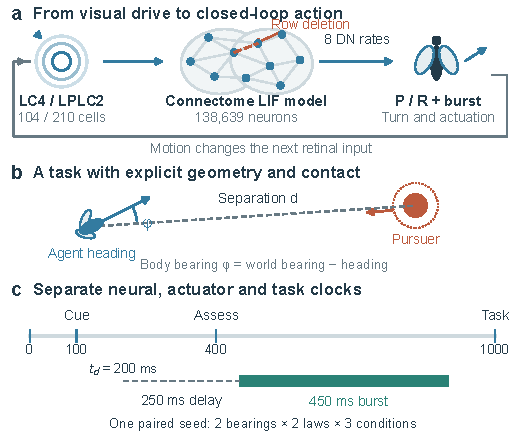
\includegraphics[width=\columnwidth]{figs/task_v9_overview.pdf}
\caption{Schematic model-to-task interface. (a) Visual drive, recurrent circuit and motion; P/R denote proportional/relay control. (b) Body-frame geometry drives input. (c) A 200-ms example decision schedules exact actuation, with next-frame control. Each seed couples twelve conditions.}
\label{fig:v9-protocol}
\end{figure}
\section{Positioning and Scope}
Shiu et al.\cite{shiu2024drosophila} connect anatomical wiring to executable sensorimotor hypotheses. An's sparsification study\cite{an2026sparse} varies connection strength, placement, state and task; Jo\cite{jo2026simulating} reports neural and virtual-arena responses to connectome damage. These works already establish context- and endpoint-dependent function. Our question concerns source-auditable pairing, sampled-data actuation and same-record exposure estimands in a prospective assessment, rather than a new claim that endpoint choice matters.

SpikeFI\cite{spyrou2024spikefi} and SpikingJET\cite{gogebakan2024spikingjet} provide SNN injection frameworks with application evaluation. NeuroBench\cite{yik2023neurobench} and embodied-agent benchmarking\cite{dangelo2026embodied} motivate separate functional and resource measurements. Here the comparisons rescore our own generated records; neither injector framework is executed as a benchmark. Physical neutron tests\cite{nijsink2026neutrons} illustrate the additional evidence needed to connect software fault models to hardware. Our weighted-row deletions have no calibrated physical upset rate, power or area interpretation.

\begin{figure*}[t]
\centering
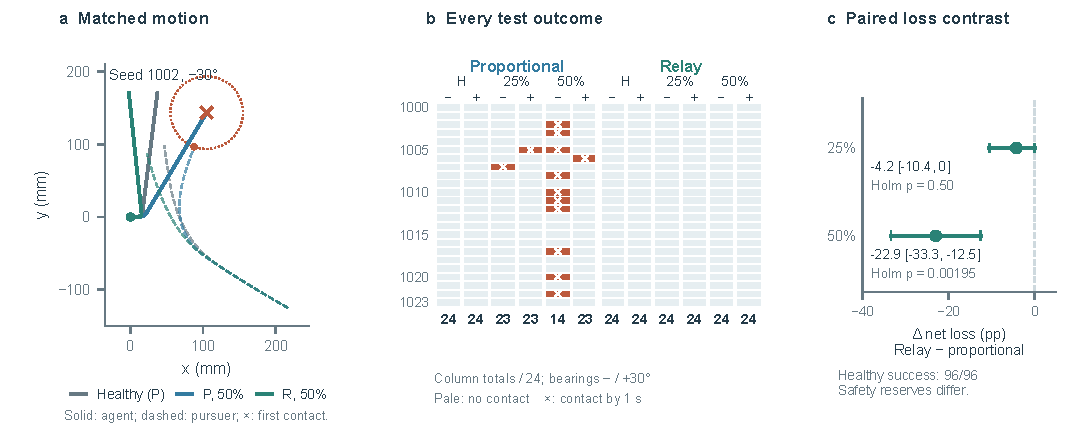
\includegraphics[width=\textwidth]{figs/task_v9_outcomes.pdf}
\caption{Feedback and task loss. (a) Actual matched paths for seed 1002, $-30^\circ$, the first seed-ordered proportional 50\%-deletion collision, shown descriptively. Solid/dashed: agent/pursuer; paths stop at first contact, with 50-mm dotted contact radius. (b) All 288 outcomes in 24 seed rows; column totals are successes/24. Bearings, laws and doses within each seed are paired. (c) Registered relay-minus-proportional net-loss contrasts, 95\% whole-seed bootstrap intervals and Holm-adjusted $p$. Healthy safety reserves differ.}
\label{fig:v9-outcomes}
\end{figure*}
\section{Paired Closed-Loop Assessment Protocol}
\label{sec:protocol}
\subsection{Substrate and Randomness}
The released FlyWire v783 graph has 138,639 neurons and 15,091,983 signed connection-table rows, each representing multiple contacts. We use the Shiu LIF parameterization\cite{shiu2024drosophila} in Brian~2\cite{stimberg2019brian2}, NumPy backend, 0.1\,ms steps. The original publication used v630. Sensory cells retain 2.2\,ms refractoriness, a stated stimulation variant. Initial states and unmodified weights are restored before each episode; equations and parameters accompany the source.

An assumed receptive-field map supplies geometry-dependent rates up to 150\,Hz to 104 LC4 and 210 LPLC2 cells. Other external rates are zero. Eight descending cells form a synthetic command interface. Anatomy and looming selectivity\cite{klapoetke2017looming} motivate the substrate; the map and body coupling are not validated fly behavior. Actual cell identities and map parameters are saved.

Each seed crosses both bearings, both laws and healthy/25\%/50\% deletion. Shared row variates define $w_j^{(f)}=w_j I(V_{sj}\geq f)$, giving nested masks. All contacts in a row are removed together. Separate frame-indexed uniforms generate inputs $I[U_{sk\tau i}<\lambda_{ki}\Delta t]$. Uniforms are common across conditions; realized events differ through feedback-dependent $\lambda$. Digests bind masks, uniforms, actual events, maps, sources and external tables. Seed traceability does not imply cross-platform bit identity.

\subsection{Causal Feedback and Actuation}
Body-frame bearing subtracts heading from world-relative bearing. Looming uses changes in $\alpha=\arctan(0.05/d)$ at actual separation $d$. Input begins at 100\,ms; decisions at each frame end affect the \emph{next} 20\,ms motion interval.

Twenty passive episodes (four seeds; $-60,-30,0,30,60^\circ$) fit a ridge decoder $z_k=\beta_0+\boldsymbol\beta^\top\bar{\mathbf r}_k$ of bearing/$60^\circ$, using five-frame means of eight command rates. Both laws set $\omega_k=0$ before the cue or below the 4.03125\,Hz eight-cell mean trigger level; otherwise
\begin{equation}
\omega_k=\begin{cases}
-600\operatorname{clip}(z_k,-1,1),&\text{proportional},\\
-600\operatorname{sgn}(z_k),&\text{relay},
\end{cases}\quad[\mathrm{deg/s}].
\end{equation}
The first qualifying decision $t_d$ schedules one 0.35\,m/s heading-fixed burst on $[t_d+250,t_d+700)$\,ms. Otherwise speed is 0.05\,m/s and heading is capped at $\pm100^\circ$. Motion segments split at exact actuator boundaries; positions use starting heading, updated at each segment end. A 0.3\,m/s pursuer starts 0.25\,m away and aims at the agent at each segment's beginning. First contact at distance $\leq0.05$\,m is solved inside each linear relative-motion segment.

Success means collision-free through 1\,s, not eventual escape. Walk-only segments satisfy $d_{\rm next}\leq d-0.25\delta$ ($\delta$ in seconds), so contact occurs by 0.8\,s without a burst in this plant. Failure latches at first contact; the trajectory and neural loop continue for equal 1\,s resource exposure. Post-contact activity is counterfactual accounting, not physical collision dynamics or warning data. Independent replay checks inputs, geometry, decisions, clocks and horizon state without rerunning neural dynamics.

\subsection{Paired Estimands}
Let $S_F(t),S_H(t)$ be paired network counts, and $T_F,T_H$ their contact-frame end or 1\,s. With $T_*=\min(T_F,T_H)$, distinguish
\begin{equation}
R_{\rm stop}=\frac{S_F(T_F)}{S_H(T_H)},\quad
R_{\rm common}=\frac{S_F(T_*)}{S_H(T_*)}.
\end{equation}
Fixed 400\,ms and 1\,s ratios are separate estimands. The former precedes all contacts; common duration remains outcome-dependent and does not equate sensory histories. For binary outcomes, report loss $Y_H(1-Y_F)$, gain $(1-Y_H)Y_F$ and net loss $D=Y_H-Y_F$. The controller interaction is $D_{\rm relay}-D_{\rm proportional}$, averaging bearings within seed.

\subsection{Validation, Warnings and Inference}
An initial controller failed its declared capability screen; all attempts are retained. Final calibration passed on eight new healthy validation clusters, 8/8 per law/bearing. A two-cluster fault screen was developmental. Core testing uses 24 new clusters (288 episodes); eight separate $\pm45^\circ$ clusters test angle transfer. Parameters, thresholds and stopping rules were frozen before both tests.

Warnings use only data through 400\,ms: low mean command rate, an upper activity limit, and $|\log(S/\tilde S_H)|$ against law/side-specific healthy medians. A held-command forecast uses current geometry, neural turn command and pending burst; absent a trigger it assumes the earliest next-frame decision. A same-state actuator baseline sets future turn to zero. Both have exact simulated geometry, not implemented sensors or reachability guarantees. Lower fifth-percentile command/clearance and upper 95th-percentile log-score thresholds use all healthy validation records. Cutoffs are 5.833\,Hz (100--400\,ms command mean), activity ratios outside $[0.844,1.185]$, and predicted clearance below 18.77/18.55\,mm for held-command/schedule forecasts. The upper resource limit is $2\tilde S_H$. Healthy flag calibration does not guarantee task false-alarm rates.

All test records contribute sensitivity, specificity, false alarms and misses against contact through 1\,s. Confidence intervals use 20,000 whole-seed percentile resamples, RNG 20261022. Controller sign-flip sensitivity assumes a symmetric cluster null, Holm-adjusted over two doses. Fixed 800/900/1000\,ms task horizons are repeated observations, not new replicates. No test tuning, seed replacement or efficacy stopping is permitted. Inference remains conditional on one model, map and task.

\section{Independent Test Results}
\subsection{Fault Loss Depends on Feedback}
All 96 healthy core episodes succeed: 24/24 for each law/bearing in Fig.~\ref{fig:v9-outcomes}. At 25\% deletion, proportional control succeeds in 46/48 episodes and relay in 48/48; at 50\%, these counts are 37/48 and 48/48. There are no healthy-to-fault gains. The 50\% proportional losses are direction-dependent: 10/24 at $-30^\circ$, 1/24 at $+30^\circ$. Both healthy directions remain capable, avoiding the earlier directional floor.

The registered relay-minus-proportional net-loss contrast at 50\% is $-22.9$ percentage points (pp), 95\% cluster interval $[-33.3,-12.5]$, with 11/24 nonzero cluster contrasts. Symmetric-null sign-flip sensitivity gives raw $p=0.000977$, Holm-adjusted $p=0.00195$. At 25\%, the contrast is $-4.2$\,pp, interval $[-10.4,0]$, adjusted $p=0.50$; two nonzero clusters provide limited evidence. Relay's zero losses are observations, not zero-risk estimates. These new laws do not replicate the older six-cluster original/gated comparison, whose exploratory 25\% $p=0.25$ remains in the supplement.



A post-hoc trace diagnostic finds identical trigger times and pre-decision traces in all 144 matched law/scenario pairs. Steering is gated below the trigger threshold, so the laws first diverge after that decision. Median trigger time rises from 160 to 220\,ms under 50\% deletion for both laws; median absolute heading at precontact 400\,ms is $38.7^\circ$ for proportional control and $96.0^\circ$ for relay. Healthy median minimum clearance is 33.1 versus 41.4\,mm. Thus identical success counts do not match safety reserve or executed turning effort. This describes a timing/turning pathway, not mediation or fault-specific superiority independent of baseline margin.

\subsection{Neural Criteria Miss Task Failures}
All 400-ms assessments precede the earliest contact, 607.6\,ms. Fig.~\ref{fig:v9-warnings} scores the same 288 records against 13 later collisions and 275 successful tasks. The command-rate criterion detects only 2/13 collisions; its sensitivity interval is $[0,40.0]\%$. Two-sided activity detects 3/13 with more false alarms, and the upper activity limit detects none. At this frozen calibration, adding a lower activity cutoff still misses 10/13 collisions.

\begin{figure*}[t]
\centering
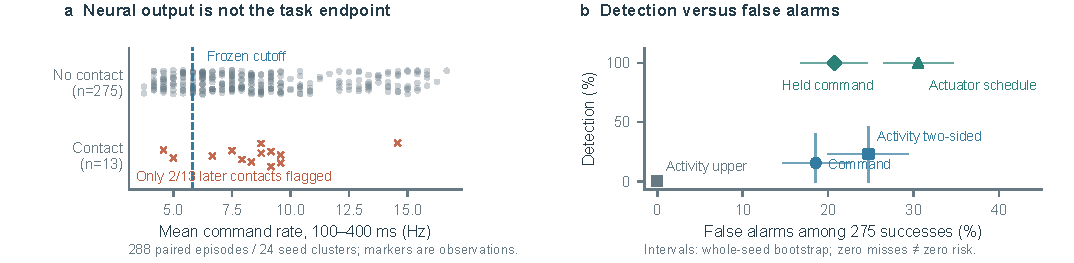
\includegraphics[width=\textwidth]{figs/task_v9_warnings.pdf}
\caption{Frozen 400-ms warnings on all core records. (a) Every command-rate observation with visual vertical jitter and the healthy-validation cutoff. (b) Detection among 13 collisions versus false alarms among 275 successes; 95\% whole-seed bootstrap intervals. Geometric forecasts use exact state; zero misses do not establish zero risk. Complete confusion counts are in the supplement.}
\label{fig:v9-warnings}
\end{figure*}

Both geometry-informed forecasts detect 13/13 collisions. Holding the current neural turn command reduces false alarms from 84 to 57 relative to the same-state zero-future-turn baseline. A secondary descriptive paired analysis gives a specificity gain of 9.8\,pp, interval $[6.6,13.4]$. Its remaining 20.7\% false-alarm rate and exact-state information limit practical interpretation. Zero observed misses yield a degenerate bootstrap interval; the one-sided 95\% bound on any miss in a new, identically defined seed cluster is 11.7\%, not a conditional FNR guarantee. This candidate is not a validated protection algorithm.

\subsection{Prespecified Angle Transfer}
Eight new $\pm45^\circ$ seed clusters retain the frozen map, laws and thresholds. All 32 healthy episodes and all 32 25\%-deletion episodes succeed. At 50\%, proportional control succeeds in 14/16 and relay in 16/16; both losses occur at negative bearing. The relay-minus-proportional contrast is $-12.5$\,pp, interval $[-31.3,0]$. This small stress cohort is not pooled with the core and does not establish a precise replication. Of two collisions, command rate flags one, two-sided activity none, and both forecasts two; held-command/schedule false alarms are 11/94 and 21/94 successful tasks. With only two failure clusters, warning sensitivity remains poorly constrained.

\subsection{Separate Action-Interface Check}
An additional eight-seed diagnostic was registered after core launch and remains separate from its inference. On 64 new healthy-network episodes, normal proportional/relay control each succeeds in 16/16; turning disabled with burst triggering retained succeeds in 0/16, and both neural actions disabled in 0/16. Baseline walking remains active. These controls support action dependence in this plant; they do not establish connectome-specific superiority or separately isolate burst effects. The walk-only feasibility bound in Methods explains why the latter failure is partly constructed.

\subsection{Horizon and Exposure Have Distinct Effects}
Only two collisions occur by 800 or 900\,ms, versus 13 by 1\,s. The 50\% controller contrast is therefore $-4.2$\,pp at the earlier horizons, versus $-22.9$\,pp at 1\,s. These are repeated observations, not extra samples; the declared horizon materially changes task loss.

In contrast, duration matching leaves every group median spike ratio unchanged. At 50\% deletion, stopped/common medians are 1.505 for proportional control and 1.257 for relay; every pair changes by less than 0.00325. The large historical stopped/common difference does not recur here. Proportional 50\% activity has median ratio 0.981 at 400\,ms and 1.505 over 1\,s, illustrating distinct resource windows. Full-horizon post-contact continuation is not prospective warning evidence.

\section{Executable Evidence and Audit Cost}
One JSON file per seed/bearing/law/fault records frames and actuator segments. Source, map, calibration and input-digest bindings reject incomplete or mixed matrices. Independent replay reconstructs geometry, decisions and inputs without importing the task implementation or loading the connectome; separate arithmetic checks verify cluster effects and warning denominators. Mutation tests reject inconsistent headings, bursts and horizon flags and confirm that prefix metrics ignore future outcomes. A tiny Brian~2 test checks episode-state and fault-weight restoration.

The core neural campaign takes 14,393\,s with three CPU workers; median episode wall time is 145.5\,s. Independent trace/input replay takes 34.4\,s. These perform different work: replay consumes recorded neural outputs and does not certify neural-state correctness or establish a simulation speedup. No hardware energy or area is inferred.

The matched package supplies raw JSON/CSV, generating snapshots, local registrations, TeX, figures and checksums; external tables remain separate. Registrations are not externally timestamped. A logged post-registration CSV fix only separates numeric-margin and Boolean-warning columns; frozen sources and raw records remain intact. Reanalysis/replay needs no new neural execution. Public main alone may predate this revision.

\section{Implications and Limits}
The same functional deletion mask can receive different task-level fault labels under two healthy-capable feedback laws. A neural threshold and a task requirement should therefore be reported separately, with actuator schedule, horizon and healthy safety reserve attached. At the tested calibration, a two-sided activity control also leaves substantial misses.

Evidence remains conditional on one v783 graph, one assumed visual map and a simple finite-horizon pursuit task. Healthy safety margins and turning effort are not matched; the law contrast does not isolate fault-specific tolerance from nominal reserve. The fixed rules are not optimized classifiers; the twofold spike envelope is not an established resource budget. Forecasts use more information than neural counts and retain substantial false alarms. Sparse failure clusters and fixed calibration limit uncertainty estimates. Row deletion is uncalibrated to physical bit errors; energy, area, real-time execution and biological tolerance are not established.

\section{Conclusion}
An auditable paired assessment separates feedback-dependent task loss from neural-rate and activity criteria in a large connectome SNN. Independent evidence supports a 50\% deletion contrast at the specified one-second endpoint; the 25\% contrast remains uncertain and stopped-duration matching has little effect in the new cohort. The reusable result is a source-bound assessment and replay workflow with explicit task, timing and resource endpoints.

\FloatBarrier
\clearpage
\bibliographystyle{IEEEtran}
\bibliography{refs}
\end{document}
